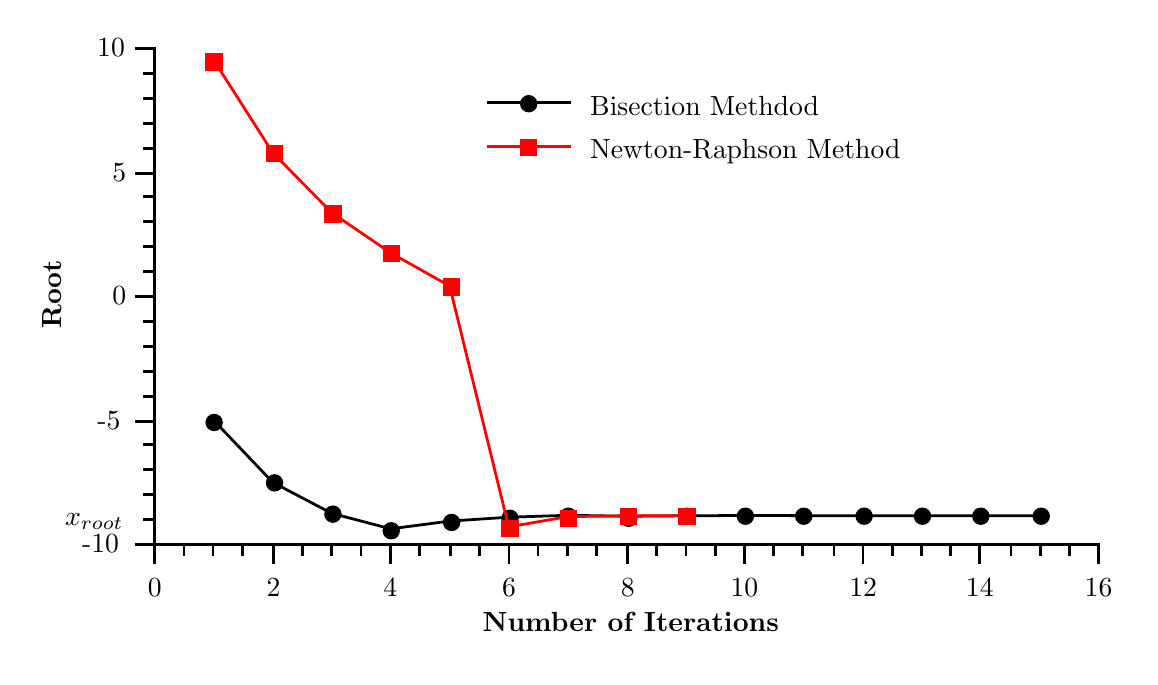
\begin{tikzpicture}{0pt}{0pt}{529pt}{302pt}
	\clip(0pt,302pt) -- (398.238pt,302pt) -- (398.238pt,74.6506pt) -- (0pt,74.6506pt) -- (0pt,302pt);
\begin{scope}
	\clip(45.9216pt,294.472pt) -- (386.946pt,294.472pt) -- (386.946pt,115.303pt) -- (45.9216pt,115.303pt) -- (45.9216pt,294.472pt);
	\color[rgb]{0,0,0}
	\draw[line width=1pt, line join=miter, line cap=rect](67.2356pt,160.095pt) -- (88.5496pt,137.699pt) -- (109.864pt,126.501pt) -- (131.178pt,120.902pt) -- (152.492pt,123.701pt) -- (173.806pt,125.101pt) -- (195.12pt,125.801pt) -- (216.434pt,125.451pt) -- (237.748pt,125.626pt) -- (259.062pt,125.713pt) -- (280.376pt,125.669pt) -- (301.69pt,125.648pt) -- (323.004pt,125.637pt) -- (344.318pt,125.642pt) -- (365.632pt,125.639pt);
	\color[rgb]{0,0,0}
	\fill(67.3767pt,159.342pt) ellipse (2.63484pt and 2.63484pt);
	\draw[line width=1pt, line join=miter, line cap=rect](67.3767pt,159.342pt) ellipse (2.63484pt and 2.63484pt);
	\fill(89.2083pt,137.51pt) ellipse (2.63484pt and 2.63484pt);
	\draw[line width=1pt, line join=miter, line cap=rect](89.2083pt,137.51pt) ellipse (2.63484pt and 2.63484pt);
	\fill(110.287pt,126.218pt) ellipse (2.63484pt and 2.63484pt);
	\draw[line width=1pt, line join=miter, line cap=rect](110.287pt,126.218pt) ellipse (2.63484pt and 2.63484pt);
	\fill(131.366pt,120.196pt) ellipse (2.63484pt and 2.63484pt);
	\draw[line width=1pt, line join=miter, line cap=rect](131.366pt,120.196pt) ellipse (2.63484pt and 2.63484pt);
	\fill(153.197pt,123.207pt) ellipse (2.63484pt and 2.63484pt);
	\draw[line width=1pt, line join=miter, line cap=rect](153.197pt,123.207pt) ellipse (2.63484pt and 2.63484pt);
	\fill(174.276pt,124.713pt) ellipse (2.63484pt and 2.63484pt);
	\draw[line width=1pt, line join=miter, line cap=rect](174.276pt,124.713pt) ellipse (2.63484pt and 2.63484pt);
	\fill(195.355pt,125.465pt) ellipse (2.63484pt and 2.63484pt);
	\draw[line width=1pt, line join=miter, line cap=rect](195.355pt,125.465pt) ellipse (2.63484pt and 2.63484pt);
	\fill(217.186pt,124.713pt) ellipse (2.63484pt and 2.63484pt);
	\draw[line width=1pt, line join=miter, line cap=rect](217.186pt,124.713pt) ellipse (2.63484pt and 2.63484pt);
	\fill(238.265pt,125.465pt) ellipse (2.63484pt and 2.63484pt);
	\draw[line width=1pt, line join=miter, line cap=rect](238.265pt,125.465pt) ellipse (2.63484pt and 2.63484pt);
	\fill(259.344pt,125.465pt) ellipse (2.63484pt and 2.63484pt);
	\draw[line width=1pt, line join=miter, line cap=rect](259.344pt,125.465pt) ellipse (2.63484pt and 2.63484pt);
	\fill(280.423pt,125.465pt) ellipse (2.63484pt and 2.63484pt);
	\draw[line width=1pt, line join=miter, line cap=rect](280.423pt,125.465pt) ellipse (2.63484pt and 2.63484pt);
	\fill(302.254pt,125.465pt) ellipse (2.63484pt and 2.63484pt);
	\draw[line width=1pt, line join=miter, line cap=rect](302.254pt,125.465pt) ellipse (2.63484pt and 2.63484pt);
	\fill(323.333pt,125.465pt) ellipse (2.63484pt and 2.63484pt);
	\draw[line width=1pt, line join=miter, line cap=rect](323.333pt,125.465pt) ellipse (2.63484pt and 2.63484pt);
	\fill(344.412pt,125.465pt) ellipse (2.63484pt and 2.63484pt);
	\draw[line width=1pt, line join=miter, line cap=rect](344.412pt,125.465pt) ellipse (2.63484pt and 2.63484pt);
	\fill(366.243pt,125.465pt) ellipse (2.63484pt and 2.63484pt);
	\draw[line width=1pt, line join=miter, line cap=rect](366.243pt,125.465pt) ellipse (2.63484pt and 2.63484pt);
	\color[rgb]{1,0,0}
	\draw[line width=1pt, line join=miter, line cap=rect](67.2356pt,290.233pt) -- (88.5496pt,256.827pt) -- (109.864pt,235.129pt) -- (131.178pt,220.619pt) -- (152.492pt,208.626pt) -- (173.806pt,121.598pt) -- (195.12pt,125.302pt) -- (216.434pt,125.635pt) -- (237.748pt,125.638pt);
	\fill(64.7419pt,292.213pt) -- (70.0116pt,292.213pt) -- (70.0116pt,286.944pt) -- (64.7419pt,286.944pt) -- (64.7419pt,292.213pt);
	\draw[line width=1pt, line join=miter, line cap=rect](64.7419pt,292.213pt) -- (70.0116pt,292.213pt) -- (70.0116pt,286.944pt) -- (64.7419pt,286.944pt) -- (64.7419pt,292.213pt);
	\fill(86.5734pt,259.09pt) -- (91.8431pt,259.09pt) -- (91.8431pt,253.82pt) -- (86.5734pt,253.82pt) -- (86.5734pt,259.09pt);
	\draw[line width=1pt, line join=miter, line cap=rect](86.5734pt,259.09pt) -- (91.8431pt,259.09pt) -- (91.8431pt,253.82pt) -- (86.5734pt,253.82pt) -- (86.5734pt,259.09pt);
	\fill(107.652pt,237.258pt) -- (112.922pt,237.258pt) -- (112.922pt,231.988pt) -- (107.652pt,231.988pt) -- (107.652pt,237.258pt);
	\draw[line width=1pt, line join=miter, line cap=rect](107.652pt,237.258pt) -- (112.922pt,237.258pt) -- (112.922pt,231.988pt) -- (107.652pt,231.988pt) -- (107.652pt,237.258pt);
	\fill(128.731pt,222.955pt) -- (134.001pt,222.955pt) -- (134.001pt,217.685pt) -- (128.731pt,217.685pt) -- (128.731pt,222.955pt);
	\draw[line width=1pt, line join=miter, line cap=rect](128.731pt,222.955pt) -- (134.001pt,222.955pt) -- (134.001pt,217.685pt) -- (128.731pt,217.685pt) -- (128.731pt,222.955pt);
	\fill(150.562pt,210.91pt) -- (155.832pt,210.91pt) -- (155.832pt,205.64pt) -- (150.562pt,205.64pt) -- (150.562pt,210.91pt);
	\draw[line width=1pt, line join=miter, line cap=rect](150.562pt,210.91pt) -- (155.832pt,210.91pt) -- (155.832pt,205.64pt) -- (150.562pt,205.64pt) -- (150.562pt,210.91pt);
	\fill(171.641pt,123.583pt) -- (176.911pt,123.583pt) -- (176.911pt,118.314pt) -- (171.641pt,118.314pt) -- (171.641pt,123.583pt);
	\draw[line width=1pt, line join=miter, line cap=rect](171.641pt,123.583pt) -- (176.911pt,123.583pt) -- (176.911pt,118.314pt) -- (171.641pt,118.314pt) -- (171.641pt,123.583pt);
	\fill(192.72pt,127.348pt) -- (197.99pt,127.348pt) -- (197.99pt,122.078pt) -- (192.72pt,122.078pt) -- (192.72pt,127.348pt);
	\draw[line width=1pt, line join=miter, line cap=rect](192.72pt,127.348pt) -- (197.99pt,127.348pt) -- (197.99pt,122.078pt) -- (192.72pt,122.078pt) -- (192.72pt,127.348pt);
	\fill(214.552pt,128.1pt) -- (219.821pt,128.1pt) -- (219.821pt,122.831pt) -- (214.552pt,122.831pt) -- (214.552pt,128.1pt);
	\draw[line width=1pt, line join=miter, line cap=rect](214.552pt,128.1pt) -- (219.821pt,128.1pt) -- (219.821pt,122.831pt) -- (214.552pt,122.831pt) -- (214.552pt,128.1pt);
	\fill(235.63pt,128.1pt) -- (240.9pt,128.1pt) -- (240.9pt,122.831pt) -- (235.63pt,122.831pt) -- (235.63pt,128.1pt);
	\draw[line width=1pt, line join=miter, line cap=rect](235.63pt,128.1pt) -- (240.9pt,128.1pt) -- (240.9pt,122.831pt) -- (235.63pt,122.831pt) -- (235.63pt,128.1pt);
\end{scope}
\begin{scope}
	\color[rgb]{0,0,0}
	\pgftext[center, base, at={\pgfpoint{12.045pt}{205.64pt}},rotate=90]{\textbf{Root}}
	\color[rgb]{0,0,0}
	\pgftext[center, base, at={\pgfpoint{26.3484pt}{112.291pt}}]{-10}
	\pgftext[center, base, at={\pgfpoint{29.3597pt}{156.707pt}}]{-5}
	\pgftext[center, base, at={\pgfpoint{33.1238pt}{201.876pt}}]{0}
	\pgftext[center, base, at={\pgfpoint{33.1238pt}{246.292pt}}]{5}
	\pgftext[center, base, at={\pgfpoint{30.1125pt}{291.461pt}}]{10}
	\draw[line width=1pt, line join=bevel, line cap=rect](45.9216pt,124.336pt) -- (42.1575pt,124.336pt);
	\draw[line width=1pt, line join=bevel, line cap=rect](45.9216pt,133.37pt) -- (42.1575pt,133.37pt);
	\draw[line width=1pt, line join=bevel, line cap=rect](45.9216pt,142.404pt) -- (42.1575pt,142.404pt);
	\draw[line width=1pt, line join=bevel, line cap=rect](45.9216pt,151.438pt) -- (42.1575pt,151.438pt);
	\draw[line width=1pt, line join=bevel, line cap=rect](45.9216pt,168.752pt) -- (42.1575pt,168.752pt);
	\draw[line width=1pt, line join=bevel, line cap=rect](45.9216pt,177.786pt) -- (42.1575pt,177.786pt);
	\draw[line width=1pt, line join=bevel, line cap=rect](45.9216pt,186.82pt) -- (42.1575pt,186.82pt);
	\draw[line width=1pt, line join=bevel, line cap=rect](45.9216pt,195.853pt) -- (42.1575pt,195.853pt);
	\draw[line width=1pt, line join=bevel, line cap=rect](45.9216pt,213.921pt) -- (42.1575pt,213.921pt);
	\draw[line width=1pt, line join=bevel, line cap=rect](45.9216pt,222.955pt) -- (42.1575pt,222.955pt);
	\draw[line width=1pt, line join=bevel, line cap=rect](45.9216pt,231.988pt) -- (42.1575pt,231.988pt);
	\draw[line width=1pt, line join=bevel, line cap=rect](45.9216pt,241.022pt) -- (42.1575pt,241.022pt);
	\draw[line width=1pt, line join=bevel, line cap=rect](45.9216pt,258.337pt) -- (42.1575pt,258.337pt);
	\draw[line width=1pt, line join=bevel, line cap=rect](45.9216pt,267.371pt) -- (42.1575pt,267.371pt);
	\draw[line width=1pt, line join=bevel, line cap=rect](45.9216pt,276.404pt) -- (42.1575pt,276.404pt);
	\draw[line width=1pt, line join=bevel, line cap=rect](45.9216pt,285.438pt) -- (42.1575pt,285.438pt);
	\draw[line width=1pt, line join=bevel, line cap=rect](45.9216pt,115.303pt) -- (39.1462pt,115.303pt);
	\draw[line width=1pt, line join=bevel, line cap=rect](45.9216pt,159.718pt) -- (39.1462pt,159.718pt);
	\draw[line width=1pt, line join=bevel, line cap=rect](45.9216pt,204.887pt) -- (39.1462pt,204.887pt);
	\draw[line width=1pt, line join=bevel, line cap=rect](45.9216pt,249.303pt) -- (39.1462pt,249.303pt);
	\draw[line width=1pt, line join=bevel, line cap=rect](45.9216pt,294.472pt) -- (39.1462pt,294.472pt);
	\draw[line width=1pt, line join=bevel, line cap=rect](45.9216pt,294.472pt) -- (45.9216pt,115.303pt);
	\pgftext[center, base, at={\pgfpoint{217.939pt}{83.6844pt}}]{\textbf{Number of Iterations}}
	\pgftext[center, base, at={\pgfpoint{45.9216pt}{96.4822pt}}]{0}
	\pgftext[center, base, at={\pgfpoint{88.8319pt}{96.4822pt}}]{2}
	\pgftext[center, base, at={\pgfpoint{130.989pt}{96.4822pt}}]{4}
	\pgftext[center, base, at={\pgfpoint{173.9pt}{96.4822pt}}]{6}
	\pgftext[center, base, at={\pgfpoint{216.81pt}{96.4822pt}}]{8}
	\pgftext[center, base, at={\pgfpoint{258.967pt}{96.4822pt}}]{10}
	\pgftext[center, base, at={\pgfpoint{301.878pt}{96.4822pt}}]{12}
	\pgftext[center, base, at={\pgfpoint{344.035pt}{96.4822pt}}]{14}
	\pgftext[center, base, at={\pgfpoint{386.946pt}{96.4822pt}}]{16}
	\draw[line width=1pt, line join=bevel, line cap=rect](56.4609pt,115.303pt) -- (56.4609pt,111.538pt);
	\draw[line width=1pt, line join=bevel, line cap=rect](77.5397pt,115.303pt) -- (77.5397pt,111.538pt);
	\draw[line width=1pt, line join=bevel, line cap=rect](99.3712pt,115.303pt) -- (99.3712pt,111.538pt);
	\draw[line width=1pt, line join=bevel, line cap=rect](120.45pt,115.303pt) -- (120.45pt,111.538pt);
	\draw[line width=1pt, line join=bevel, line cap=rect](141.529pt,115.303pt) -- (141.529pt,111.538pt);
	\draw[line width=1pt, line join=bevel, line cap=rect](163.36pt,115.303pt) -- (163.36pt,111.538pt);
	\draw[line width=1pt, line join=bevel, line cap=rect](184.439pt,115.303pt) -- (184.439pt,111.538pt);
	\draw[line width=1pt, line join=bevel, line cap=rect](205.518pt,115.303pt) -- (205.518pt,111.538pt);
	\draw[line width=1pt, line join=bevel, line cap=rect](227.349pt,115.303pt) -- (227.349pt,111.538pt);
	\draw[line width=1pt, line join=bevel, line cap=rect](248.428pt,115.303pt) -- (248.428pt,111.538pt);
	\draw[line width=1pt, line join=bevel, line cap=rect](269.507pt,115.303pt) -- (269.507pt,111.538pt);
	\draw[line width=1pt, line join=bevel, line cap=rect](291.338pt,115.303pt) -- (291.338pt,111.538pt);
	\draw[line width=1pt, line join=bevel, line cap=rect](312.417pt,115.303pt) -- (312.417pt,111.538pt);
	\draw[line width=1pt, line join=bevel, line cap=rect](333.496pt,115.303pt) -- (333.496pt,111.538pt);
	\draw[line width=1pt, line join=bevel, line cap=rect](355.327pt,115.303pt) -- (355.327pt,111.538pt);
	\draw[line width=1pt, line join=bevel, line cap=rect](376.406pt,115.303pt) -- (376.406pt,111.538pt);
	\draw[line width=1pt, line join=bevel, line cap=rect](67.0003pt,115.303pt) -- (67.0003pt,111.538pt);
	\draw[line width=1pt, line join=bevel, line cap=rect](109.911pt,115.303pt) -- (109.911pt,111.538pt);
	\draw[line width=1pt, line join=bevel, line cap=rect](152.821pt,115.303pt) -- (152.821pt,111.538pt);
	\draw[line width=1pt, line join=bevel, line cap=rect](194.978pt,115.303pt) -- (194.978pt,111.538pt);
	\draw[line width=1pt, line join=bevel, line cap=rect](237.889pt,115.303pt) -- (237.889pt,111.538pt);
	\draw[line width=1pt, line join=bevel, line cap=rect](280.046pt,115.303pt) -- (280.046pt,111.538pt);
	\draw[line width=1pt, line join=bevel, line cap=rect](322.957pt,115.303pt) -- (322.957pt,111.538pt);
	\draw[line width=1pt, line join=bevel, line cap=rect](365.867pt,115.303pt) -- (365.867pt,111.538pt);
	\draw[line width=1pt, line join=bevel, line cap=rect](45.9216pt,115.303pt) -- (45.9216pt,108.527pt);
	\draw[line width=1pt, line join=bevel, line cap=rect](88.8319pt,115.303pt) -- (88.8319pt,108.527pt);
	\draw[line width=1pt, line join=bevel, line cap=rect](130.989pt,115.303pt) -- (130.989pt,108.527pt);
	\draw[line width=1pt, line join=bevel, line cap=rect](173.9pt,115.303pt) -- (173.9pt,108.527pt);
	\draw[line width=1pt, line join=bevel, line cap=rect](216.81pt,115.303pt) -- (216.81pt,108.527pt);
	\draw[line width=1pt, line join=bevel, line cap=rect](258.967pt,115.303pt) -- (258.967pt,108.527pt);
	\draw[line width=1pt, line join=bevel, line cap=rect](301.878pt,115.303pt) -- (301.878pt,108.527pt);
	\draw[line width=1pt, line join=bevel, line cap=rect](344.035pt,115.303pt) -- (344.035pt,108.527pt);
	\draw[line width=1pt, line join=bevel, line cap=rect](386.946pt,115.303pt) -- (386.946pt,108.527pt);
	\draw[line width=1pt, line join=bevel, line cap=rect](45.9216pt,115.303pt) -- (386.946pt,115.303pt);
	\draw[line width=1pt, line join=miter, line cap=rect](166.372pt,274.899pt) -- (195.731pt,274.899pt);
	\fill(181.051pt,274.522pt) ellipse (2.63484pt and 2.63484pt);
	\draw[line width=1pt, line join=miter, line cap=rect](181.051pt,274.522pt) ellipse (2.63484pt and 2.63484pt);
	\pgftext[left, base, at={\pgfpoint{203.259pt}{270.382pt}}]{Bisection Methdod}
	\color[rgb]{1,0,0}
	\draw[line width=1pt, line join=miter, line cap=rect](166.372pt,259.09pt) -- (195.731pt,259.09pt);
	\fill(178.417pt,261.348pt) -- (183.686pt,261.348pt) -- (183.686pt,256.078pt) -- (178.417pt,256.078pt) -- (178.417pt,261.348pt);
	\draw[line width=1pt, line join=miter, line cap=rect](178.417pt,261.348pt) -- (183.686pt,261.348pt) -- (183.686pt,256.078pt) -- (178.417pt,256.078pt) -- (178.417pt,261.348pt);
	\color[rgb]{0,0,0}
	\pgftext[left, base, at={\pgfpoint{203.259pt}{254.573pt}}]{Newton-Raphson Method}
	\pgftext[left, base, at={\pgfpoint{13.5506pt}{122.078pt}}]{$x_{\text{root}}$}
\end{scope}
\end{tikzpicture}
